\documentclass{article}
\usepackage{graphicx} % Required for inserting images
\usepackage{url}
\usepackage{hyperref}



\begin{document}

\title{git_assignment}
\author{Danny Cruz}
\date{October 2024}

\begin{figure}
    \centering
    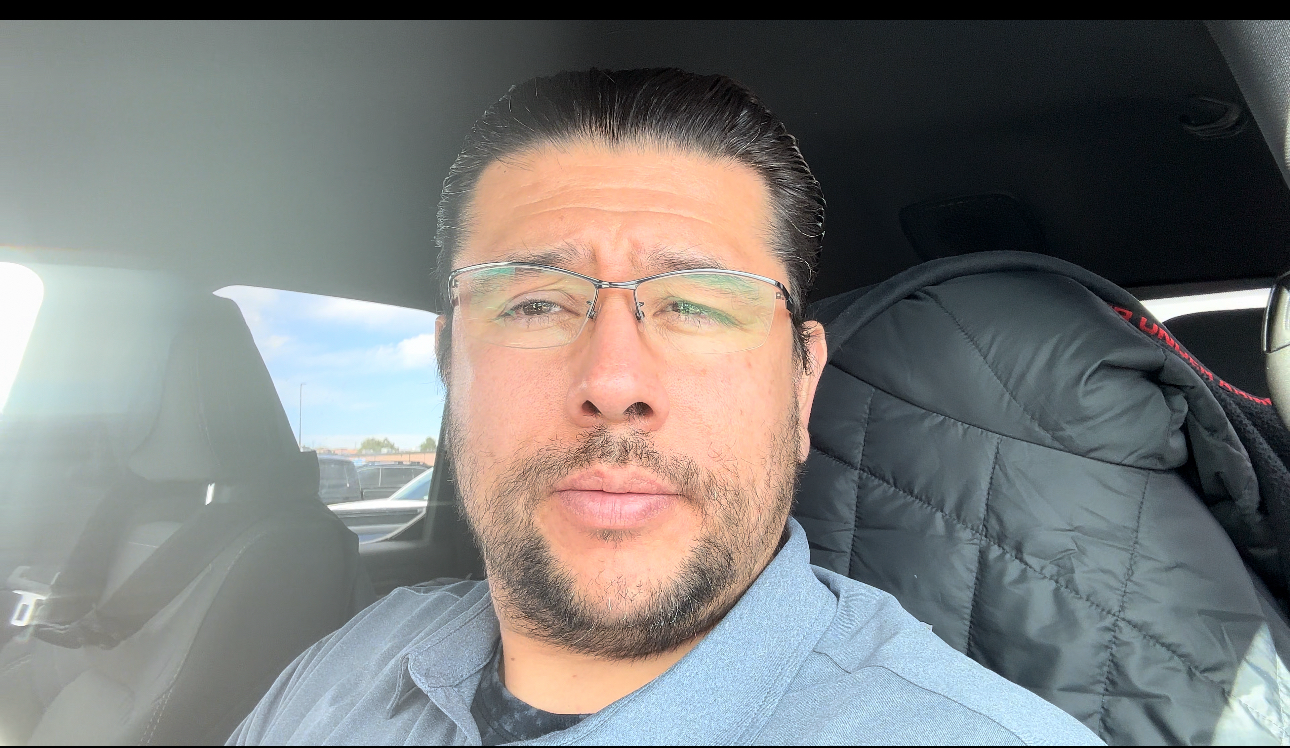
\includegraphics[width=0.5\linewidth]{images/cruz-F24.png}
    \caption{Enter Caption}
    \label{fig:enter-label}
\end{figure}

\section{My Goals for the Course}
My goals for this course is to become a proficient writer and research scientist. I want to be able to learn the basics and some advanced techniques for conducting research so that I can use the skills developed in this class through the rest of my graduate career. I hope to focus the work that I will complete on a PhD.

What I hope to learn in this course is how to conduct proper research and identify accurate experimental designs. I want to start my academic career off on the right foot. I do not want to waste effort on research that does not apply to my thesis. I have taken only two courses here at the University of Colorado, so I believe that I am still in great shape to produce research papers that apply to future requirements. 

I will eventually be working on a PhD, so this would be a step in the right direction. One of the problems that I have heard about is that people don't take this course first before they start randomly developing research papers that will not apply to their thesis. I hope to avoid that problem and take the right steps toward efficiently building up the right material for a PhD.

I am currently working on a Masters of Science in Computer Science with a focus in A.I. algorithms. My interest is in neural networks particularly the transformer NN. I hope to prepare my self for a PhD in the future by completing this class. I believe by learning how to do efficient research in the field will set me off on the right foot towards this ultimate goal. By taking this course early in my graduate career I hope to avoid doing research in areas that will not continually focus on building up to this goal.

Something personal about my self is that in my off time, I like to study various Machine Learning and Natural Language Processing algorithms in VS code using Jupiter Notebook. I have been experimenting with techniques of Data Mining as well. In my current job I am a software engineer and we are working on implementing predictive maintenance for the manufacturing machines that my company sells. We want to be able to have the machines predict when a part will most likely fail. Since this is a problem currently appearing in industry 4.0 I find its application beneficial and useful.

My most recent focus is how to apply Principal Component Analysis and a Transformer based Neural Network to the predictive maintenance problem we are working on that uses time series data. I believe by doing practical application and research experiments on these topics it will provide me with the skills and knowledge that I will need to complete my M.S. in C.S. and prepare me for working on my PhD.

\section{Code Run}

The code I chose to run is from a book called Applied Machine Learning for Engineers. The code is for detecting anomalies in bearings on an industrial machine. The link for the Github repository is located here: \href{Applied Machine Learning for Engineers}{\href{https://github.com/jeffprosise/Applied-Machine-Learning}{jeffprosise/Applied-Machine-Learning (github.com)}}

In this image we can see how we highlight when bearings begin to wear and anomaly detection is picking up a problem highlighted in red

\begin{figure}[!h]
    \centering
    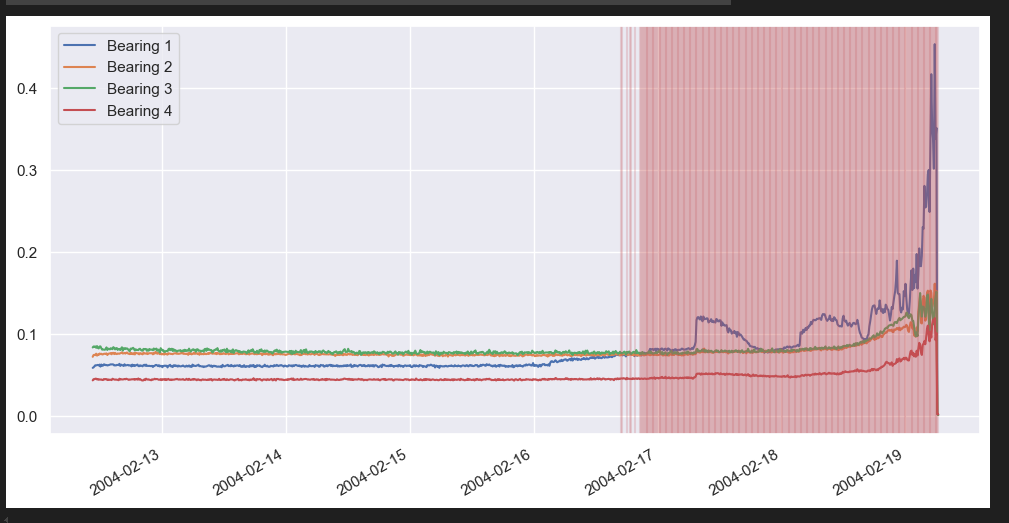
\includegraphics[width=0.5\linewidth]{images/bearing vibrations 2024-10-20.png}
    \caption{Bearing Vibrations Anomaly Detection}
    \label{fig:1}
\end{figure}


\section{Questions}

Please post any questions you have for me below.

Q1. Your work is very interesting. What exactly is predictive maintenance problem?

 \subsection    What was the most challenging part of your project?
 

\end{document}
